% SI Figure 1 of "Partners, rivals, and friendly rivals in the evolution of direct reciprocity":
% feasible payoff pairs and the two half-planes behind the theorem.  A standalone TikZ picture.
% Build: sh build.sh   (or: pdflatex SIFig1.tex)
\documentclass[tikz,border=6pt]{standalone}
\usepackage{times}
\usepackage{amsmath,amssymb}
\usetikzlibrary{arrows.meta,calc}
\newcommand{\Emax}{E_{\max}}
\begin{document}
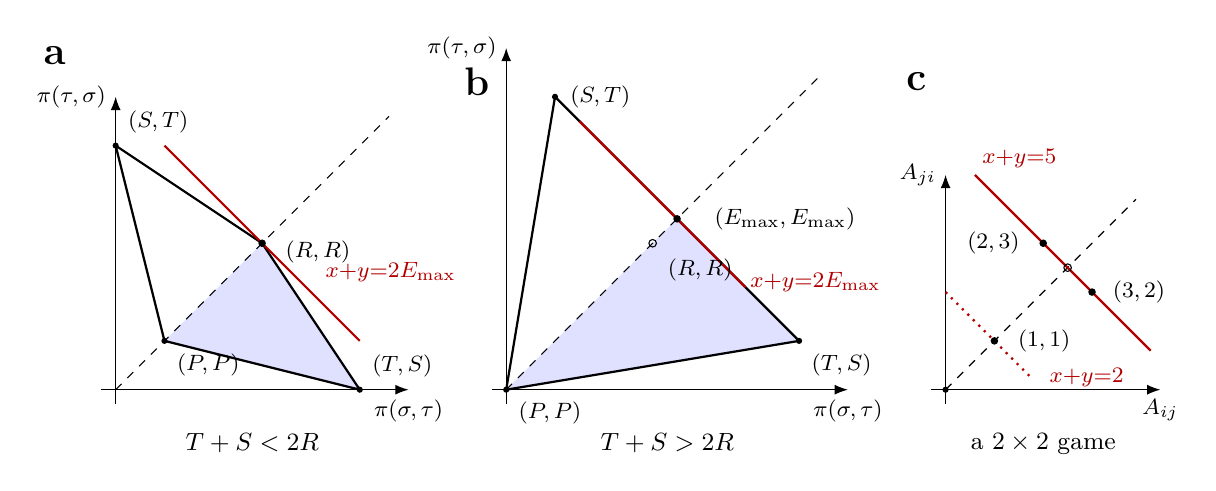
\begin{tikzpicture}[scale=0.62,>=Latex]
% ---------- panel a: below the switch line ----------
\begin{scope}
  \node[font=\Large\bfseries] at (-1.25,6.85) {a};
  \fill[blue!12] (1,1) -- (5,0) -- (3,3) -- cycle;
  \draw[->] (-0.3,0) -- (6,0) node[below] {\footnotesize $\pi(\sigma,\tau)$};
  \draw[->] (0,-0.3) -- (0,6) node[left] {\footnotesize $\pi(\tau,\sigma)$};
  \draw[thick] (1,1) -- (5,0) -- (3,3) -- (0,5) -- cycle;
  \draw[dashed] (0,0) -- (5.6,5.6);
  \draw[red!70!black,thick] (1.0,5.0) -- (5.0,1.0);
  \node[red!70!black,anchor=south west] at (4.1,2.0) {\footnotesize $x{+}y{=}2\Emax$};
  \fill (3,3) circle (2.2pt) node[right=5pt,yshift=-3pt] {\footnotesize $(R,R)$};
  \fill (0,5) circle (1.8pt) node[above right=1pt] {\footnotesize $(S,T)$};
  \fill (5,0) circle (1.8pt) node[above right=1pt] {\footnotesize $(T,S)$};
  \fill (1,1) circle (1.8pt) node[below right=1pt] {\footnotesize $(P,P)$};
  \node at (2.8,-1.1) {\small $T+S<2R$};
\end{scope}
% ---------- panel b: above the switch line ----------
\begin{scope}[xshift=8cm]
  \node[font=\Large\bfseries] at (-0.6,6.3) {b};
  \fill[blue!12] (0,0) -- (6,1) -- (3.5,3.5) -- cycle;
  \draw[->] (-0.3,0) -- (7,0) node[below] {\footnotesize $\pi(\sigma,\tau)$};
  \draw[->] (0,-0.3) -- (0,7) node[left] {\footnotesize $\pi(\tau,\sigma)$};
  \draw[thick] (0,0) -- (6,1) -- (1,6) -- cycle;
  \draw[dashed] (0,0) -- (6.4,6.4);
  \draw[red!70!black,thick] (1.5,5.5) -- (4.9,2.1);
  \node[red!70!black,anchor=north west] at (4.8,2.6) {\footnotesize $x{+}y{=}2\Emax$};
  \fill (3.5,3.5) circle (2.2pt) node[right=10pt] {\footnotesize $(\Emax,\Emax)$};
  \draw (3,3) circle (2.2pt) node[below right=2pt] {\footnotesize $(R,R)$};
  \fill (1,6) circle (1.8pt) node[right=2pt] {\footnotesize $(S,T)$};
  \fill (6,1) circle (1.8pt) node[below right=1pt] {\footnotesize $(T,S)$};
  \fill (0,0) circle (1.8pt) node[below right=1pt] {\footnotesize $(P,P)$};
  \node at (3.3,-1.1) {\small $T+S>2R$};
\end{scope}
% ---------- panel c: the 2x2 example A = (1 3; 2 0) of the SI ----------
\begin{scope}[xshift=17cm]
  \node[font=\Large\bfseries] at (-0.6,6.3) {c};
  \draw[->] (-0.3,0) -- (4.4,0) node[below] {\footnotesize $A_{ij}$};
  \draw[->] (0,-0.3) -- (0,4.4) node[left] {\footnotesize $A_{ji}$};
  \draw[dashed] (0,0) -- (3.9,3.9);
  \draw[red!70!black,thick] (0.6,4.4) -- (4.2,0.8) node[pos=0.0,above right=-1pt] {\footnotesize $x{+}y{=}5$};
  \draw[red!70!black,dotted,thick] (0,2) -- (1.75,0.25) node[right=3pt] {\footnotesize $x{+}y{=}2$};
  \fill (1,1) circle (2.2pt) node[right=5pt] {\footnotesize $(1,1)$};
  \fill (3,2) circle (2.2pt) node[right=4pt] {\footnotesize $(3,2)$};
  \fill (2,3) circle (2.2pt) node[left=5pt] {\footnotesize $(2,3)$};
  \fill (0,0) circle (1.8pt);
  \draw (2.5,2.5) circle (2.2pt);
  \node at (2.0,-1.1) {\small a $2\times2$ game};
\end{scope}
\end{tikzpicture}
\end{document}
